Since in the compressed \gls{susy} squark-neutralino model the $\met$ and jets
recoil against an \gls{isr} jet, the average jet momenta are lower than the
missing energy, thus requiring an asymmetric cut on the leading jet momentum and
$\met$ to capture this signal. Prior to deciding the signal region selections
presented in \cref{sec:event-selection} a signal region (AM1) with
$\met > 700$~GeV and leading jet $\pt > 300$~GeV was defined and compared with
the IM1 signal region. Since the final integrated luminosity cannot be known in
advance, the studies on AM1 and IM1 were carried out on a foreseen integrated
luminosity of L~=~3.3~$\ifb$. The results for these two signal regions is
presented in \cref{fig:im1_straight_comparison}. On these figure a model is
excludable if the signal strength $\mu$, depicted by the color scale in the
picture, is lower than one. The sensitivity improves for the signal region AM1
to reflect the asymmetric kinematics.
\begin{figure}[!htb]
  \centering
  \begin{subfigure}[t]{.48\linewidth}
    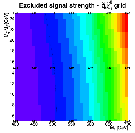
\includegraphics[width=\linewidth]{expected_im1}
    \caption{IM1.}
    \label{fig:expected_im1}
  \end{subfigure}
  \begin{subfigure}[t]{.48\linewidth}
    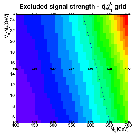
\includegraphics[width=\linewidth]{expected_straight_cut}
    \caption{AM1.}
    \label{fig:expected_straight}
  \end{subfigure}

  \begin{subfigure}[t]{.48\linewidth}
    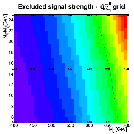
\includegraphics[width=\linewidth]{expected_shape_fit}
    \caption{Shape fit.}
    \label{fig:expected_shape}
  \end{subfigure}
  \caption{Sensitivity to the compressed SUSY models with an integrated
    luminosity of L$~=~3.3~\ifb$~in the plane defined by the squark mass
    $m_{\tilde{q}}$ and the mass difference between the squark mass and the
    lightest neutralino mass
    $\Delta m = m(\tilde{q}) - m(\tilde{\chi}_{1}^{0})$. The color scale
    reflects the lowest excludable signal strength for a particular mass
    point. The values indicated on the map indicate the actual excludable $\mu$
    values at a some specific SUSY models. The dashed line shows the limit
    between excludable and not excludable models. The theoretical uncertainties
    in the signal are not included.}
  \label{fig:im1_straight_comparison}
\end{figure}

In the AM1 signal region, models with mass gaps $\Delta m = 5$~GeV between the
squark mass and the neutralino mass, can be excluded up to squark masses of
650~GeV. At a larger mass gap of $\Delta m = 25$~GeV, squark masses up to
580~GeV are excludable.

The performance of the shape fit method was also tested on the \gls{susy}
compressed squark-neutralino model and the result is also shown in
\cref{fig:im1_straight_comparison}. The shape fit method, thanks to its
flexibility, is capable of adapting to different signal models and thus improves
the expected limits of the SUSY squark-neutralino model especially for the
largest mass gap of $\Delta m = 25$~GeV between the squark and the neutralino
masses.  \pagebreak[4]
%%% Local Variables:
%%% mode: latex
%%% TeX-master: "../search_for_DM_LED_with_ATLAS"
%%% End:
